%% ------------------------------------------------------------------
%% Numerical-illustration section, tailored to
%% "Simple Neural Networks Do Have Universal Approximation Property".
%% Uses the paper's own macros (\R, \e) and labels
%% (sec:construction, sec:kappa, th:Guliyev:str:monotone, eq:pos, eq:neg,
%%  eq:kappa:approximation).  Place e.g. just before Section~\ref{...}
%% "Concluding Remarks", or as a subsection of Section~\ref{sec:kappa:consequences}.
%% Figure file: kappa_h_comparison.png  (produced by kappa_h_compare.py).
%% ------------------------------------------------------------------
\section{A Numerical Illustration of the Construction}\label{sec:experiments}

The construction of $\kappa$ in Section~\ref{sec:kappa} is explicit, and
Corollary~\ref{th:Guliyev:str:monotone} is constructive: given a target
$f\in C([-1,1])$ it produces a single-hidden-layer, two-neuron network
$c_1\kappa(-x-d)+c_2\kappa(x+d)$ approximating $f$. To make this concrete, and to
exhibit the gap between the tailored activation $\kappa$ and a generic sigmoid at
equal (minimal) network size, we realise the construction in double precision and
measure the resulting error on two representative targets. We stress that this
serves only as an \emph{illustration} of the constructive statement; in agreement
with the discussion in the introduction, it adds no information beyond what
Corollary~\ref{th:Guliyev:str:monotone} already guarantees.

\subsection{Set-up}

We realise $\kappa$ exactly as in Sections~\ref{sec:construction}
and~\ref{sec:kappa}, with the odd scaffold
$h(t)=2\big(\tfrac{1}{1+e^{-t}}-\tfrac12\big)$ of Section~\ref{sec:construction}.
Each polynomial $p_n=p_n^{+}-p_n^{-}$ is placed in the window $[4n,4n+2]$ through
\eqref{eq:pos}--\eqref{eq:neg}, with the linear element $l_n$ taken constant and
equal to the level $h(4n+1)$ of the scaffold (permitted by the footnote to
\eqref{eq:pos}, as $p_n^{\pm}$ are strictly increasing), so that $h$ supplies
every connector between windows and both $\pm1$ tails. With $a_1^{n}=a_2^{n}=d_n^{-1}$
the decoding identity
\begin{equation}\label{eq:decode-num}
  d_n^{-1}\Big(\kappa(x+4n+1)+\kappa(-x-4n-1)\Big)=p_n(x),\qquad x\in[-1,1],
\end{equation}
holds exactly (the constant $l_n$ cancels), which is the content of
\eqref{eq:kappa}.

Given a target $f$ we take its best polynomial approximation $p$ of degree $m$ on
$[-1,1]$, encode $p$ into a window of $\kappa$, and form the two-neuron network of
Corollary~\ref{th:Guliyev:str:monotone},
\begin{equation}\label{eq:net-num}
  F(x)=c_1\,\kappa(-x-d)+c_2\,\kappa(x+d),
\end{equation}
determining $c_1,c_2$ by least squares on a uniform grid of $500$ points; the
error is then evaluated on a finer grid of $2000$ points in $[-1,1]$. For
comparison we also fit, in exactly the same way, a two-neuron network using the
standard $\tanh$ activation instead of $\kappa$.

\subsection{Targets and results}

We consider
\begin{align}
  f_1(x) &= 1+x+\tfrac{x^{2}}{2}+\tfrac{x^{3}}{6}+\tfrac{x^{4}}{24}
            +\tfrac{x^{5}}{120}+\tfrac{x^{6}}{720},\label{eq:f1num}\\[2pt]
  f_2(x) &= \frac{4x}{4+x^{2}},\label{eq:f2num}
\end{align}
on $[-1,1]$: the degree-$6$ Taylor polynomial of $e^{x}$ (encoding degree
$m=6$), and a smooth non-polynomial (rational, odd) map (encoding degree $m=14$).

Table~\ref{tab:exp} and Figure~\ref{fig:exp} report the outcome. With only
\emph{two} neurons in a single hidden layer, the network~\eqref{eq:net-num}
reproduces $f_1$ to machine precision and $f_2$ to order $10^{-9}$, whereas a
two-neuron $\tanh$ network is limited to errors of order $10^{-1}$ on the same
targets --- roughly ten orders of magnitude larger. This is exactly the effect
underlying our results: the tailored activation $\kappa$ concentrates in two
neurons the approximation power that a generic sigmoid attains only with many.
For a polynomial target ($f_1$) the approximation is exact up to round-off, since
$\kappa$ encodes polynomials verbatim through \eqref{eq:decode-num}; for a
non-polynomial target ($f_2$) the error is that of the underlying degree-$m$
polynomial approximation and decreases as $m$ grows.

\begin{table}[t]
  \centering
  \begin{tabular}{llcc}
    \hline
    Target & Activation ($2$ neurons) & max.\ error & RMS error \\
    \hline
    $f_1$ \eqref{eq:f1num} & $\kappa$ (Section~\ref{sec:kappa}) & $1.4\times10^{-13}$ & $6.1\times10^{-14}$ \\
                           & $\tanh$                            & $1.2\times10^{-1}$  & $3.6\times10^{-2}$  \\
    \hline
    $f_2$ \eqref{eq:f2num} & $\kappa$ (Section~\ref{sec:kappa}) & $3.8\times10^{-9}$  & $9.1\times10^{-10}$ \\
                           & $\tanh$                            & $6.8\times10^{-2}$  & $2.7\times10^{-2}$  \\
    \hline
  \end{tabular}
  \caption{Approximation error on $[-1,1]$ of the single-hidden-layer, two-neuron
    network~\eqref{eq:net-num} of Corollary~\ref{th:Guliyev:str:monotone}, for the
    tailored activation $\kappa$ and for the standard $\tanh$. Encoding degree
    $m=6$ for $f_1$ and $m=14$ for $f_2$.}
  \label{tab:exp}
\end{table}

\begin{figure}[t]
  \centering
  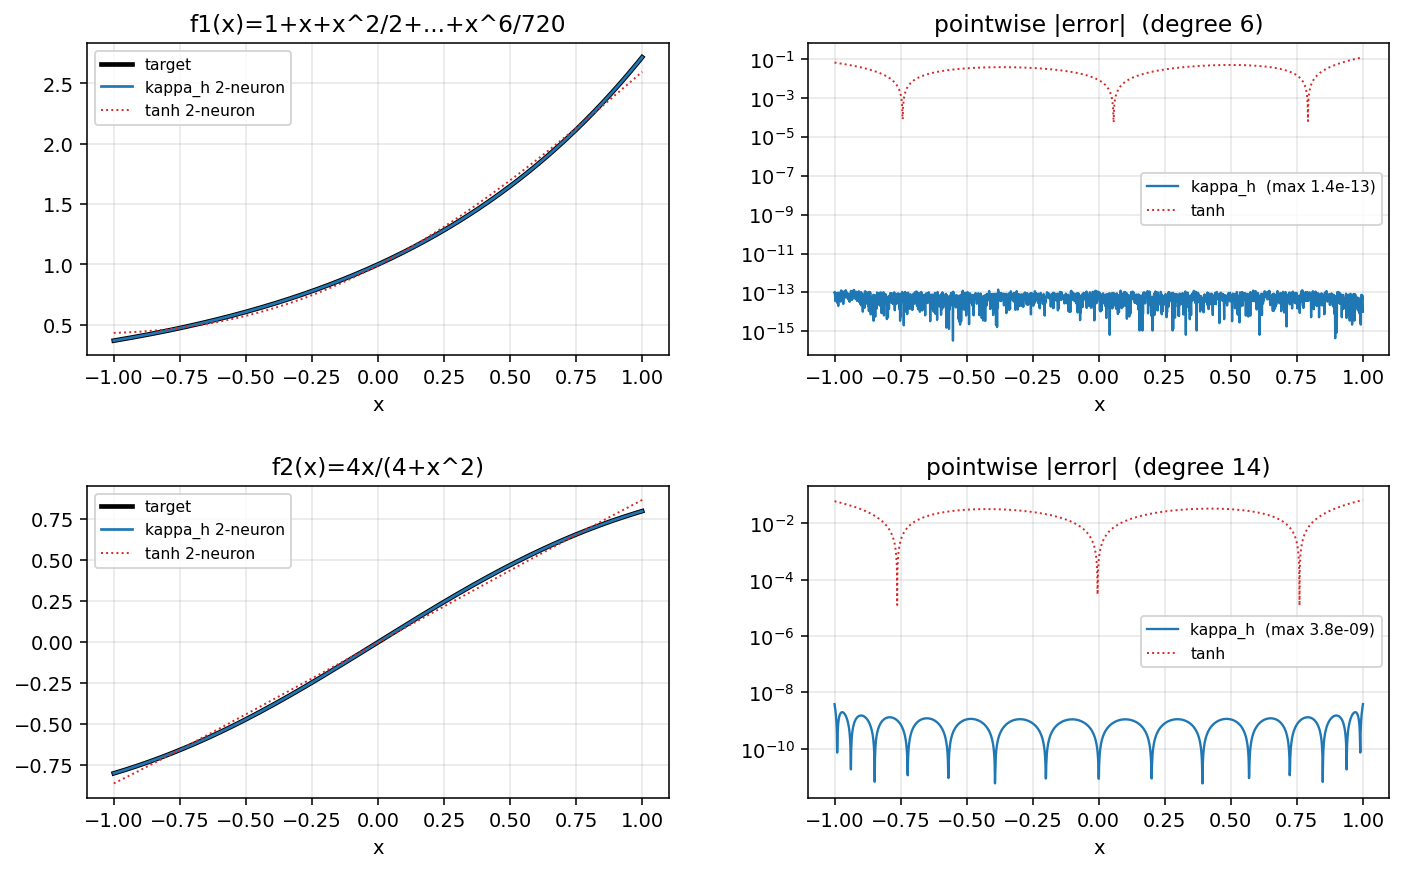
\includegraphics[width=\linewidth]{kappa_h_comparison.png}
  \caption{Two-neuron approximation of $f_1$ (top) and $f_2$ (bottom). Left:
    target versus the $\kappa$- and $\tanh$-networks. Right: pointwise absolute
    error on a logarithmic scale; the $\kappa$-network (solid) lies $8$--$12$
    orders of magnitude below the $\tanh$ baseline (dotted).}
  \label{fig:exp}
\end{figure}

\begin{remark}[On the numerical realisation]
The identity \eqref{eq:decode-num} is exact for every window index $n$ in real
arithmetic. In floating point, however, the scaffold saturates so fast that
$h(4n+1)\to1$ within machine precision already for moderate $n$; the admissible
band amplitude $d_n$, of the order of $h(4n+2)-h(4n)$, then falls below the
resolution of the floating-point grid near $1$ (so that $1+d_n$ rounds to $1$)
and the encoded polynomial is lost. A faithful double-precision realisation is
therefore restricted to small window indices; above we encode each target in the
first window, $n=1$ (shift $d=5$). This is a property of the particular scaffold
$h$ and not of the construction itself: a scaffold that saturates more slowly, or
one assembled from bounded-variation pieces of fixed vertical scale, removes the
restriction while preserving properties (i)--(iv) of $\kappa$.
\end{remark}
